\documentclass[fleqn,10pt]{article}
\usepackage[utf8]{inputenc}
\usepackage[T1]{fontenc}
\usepackage{graphicx}
\usepackage{geometry}
\usepackage{amsmath,amssymb}
\usepackage{listings}
\usepackage{xcolor}
\usepackage{tcolorbox}
\usepackage{booktabs}
\usepackage{caption}
\usepackage{amssymb}

\geometry{a4paper, margin=1in}

% Estilo para código Python
\definecolor{codegreen}{rgb}{0,0.6,0}
\definecolor{codegray}{rgb}{0.5,0.5,0.5}
\definecolor{codepurple}{rgb}{0.58,0,0.82}
\definecolor{backcolour}{rgb}{0.95,0.95,0.92}

\lstdefinestyle{pythonstyle}{
    backgroundcolor=\color{backcolour},
    commentstyle=\color{codegreen},
    keywordstyle=\color{magenta},
    numberstyle=\tiny\color{codegray},
    stringstyle=\color{codepurple},
    basicstyle=\ttfamily\footnotesize,
    breaklines=true,
    captionpos=b,
    keepspaces=true,
    tabsize=2,
    language=Python,
    showstringspaces=false,
    numbers=left,
    numbersep=5pt,
    frame=single,
    rulecolor=\color{black}
}

\begin{document}

%---------------------- portada ----------------------
\begin{titlepage}
    \centering
    \vspace*{1cm}
    {\LARGE\bfseries UNIVERSIDAD NACIONAL DE SAN ANTONIO ABAD DEL CUSCO\par}
    \vspace{0.5cm}
    {\Large FACULTAD DE INGENIERÍA ELÉCTRICA, ELECTRÓNICA, INFORMÁTICA Y MECÁNICA\par}
    \vspace{0.5cm}
    {\Large ESCUELA PROFESIONAL DE INGENIERÍA INFORMÁTICA Y DE SISTEMAS\par}
    \vfill
    \includegraphics[width=0.25\linewidth]{Escudo_UNSAAC.png}\par
    \vfill
    {\Large\bfseries CURSO: BIOINFORMÁTICA\par}
    \vspace{0.3cm}
    {\Large\bfseries TRABAJO: BÚSQUEDA DE PATRONES\par}
    \vspace{0.3cm}
    {\Large\bfseries PROFESORA: MARIA DEL PILAR VENEGAS VERGARA\par}
    \vspace{1cm}
    {\Large\bfseries ALUMNO: EFRAIN VITORINO MARÍN\par}
    {\Large\bfseries CÓDIGO: 160337\par}
    \vfill
    {\Large 2025‑I\par}
\end{titlepage}

\setcounter{page}{1}
\pagestyle{plain}
\tableofcontents
\newpage

%---------------------- contenido ----------------------
\section{Introducción Teórica}

\subsection{¿Qué es mutación?}
\textbf{Definición:}
Una mutación es un cambio en la secuencia de nucleótidos de un genoma, ya sea por sustitución, inserción, eliminación o reorganización de bases.

\bigskip
\textbf{Ejemplos:}
\begin{itemize}
    \item Sustitución: \texttt{ATG} \(\to\) \texttt{ACG} (T \(\to\) C).
    \item Inserción:    \texttt{ATG} \(\to\) \texttt{ATCG} (se inserta C).
    \item Deleción:     \texttt{ATG} \(\to\) \texttt{AG}  (se elimina T).
\end{itemize}

\textbf{Aplicaciones:}
\begin{itemize}
    \item Estudios de evolución molecular.
    \item Identificación de enfermedades genéticas.
    \item Desarrollo de resistencia a fármacos en patógenos.
\end{itemize}

\subsection{¿Qué es un k-mero esquivo?}
\textbf{Definición:}
Un \emph{k-mero esquivo} es una secuencia de longitud \(k\) que no aparece en un genoma o conjunto de datos dado, aunque habría \(\sigma^k\) posibles bajo el alfabeto de tamaño \(\sigma\).

\medskip
\begin{align}
N_{\mathrm{total}} &= \sigma^k,\\
N_{\mathrm{esquivos}} &= \sigma^k - N_{\mathrm{observados}}.
\end{align}

\textbf{Aplicaciones:}
\begin{itemize}
    \item Detección de errores en secuenciación.
    \item Identificación de regiones genómicas raras.
    \item Análisis de diversidad genética.
\end{itemize}

\subsection{Porcentaje de similitud usando Hamming}
\textbf{Definición:}
La distancia de Hamming \(D_H\) entre dos cadenas \(s_1,s_2\) de longitud \(n\) es
\[
D_H(s_1,s_2)
= \sum_{i=1}^{n} \mathbf{1}\bigl(s_1[i]\neq s_2[i]\bigr),
\]
donde \(\mathbf{1}(\cdot)\) es la función indicadora.
El porcentaje de similitud es
\[
S_H = \Bigl(1 - \tfrac{D_H}{n}\Bigr)\times 100\%.
\]

\textbf{Aplicaciones:}
\begin{itemize}
    \item Alineamiento de reads de ADN.
    \item Corrección de errores en secuenciación.
\end{itemize}

\subsection{Porcentaje de similitud usando Levenshtein}
\textbf{Definición:}
La distancia de Levenshtein \(D_L\) es el mínimo número de inserciones, eliminaciones o sustituciones para convertir \(s_1\) en \(s_2\). Se calcula con la recurrencia
\[
D_{i,j}=
\begin{cases}
\max(i,j), & \min(i,j)=0,\\[6pt]
\min\bigl\{
    D_{i-1,j}+1,\;
    D_{i,j-1}+1,\;
    D_{i-1,j-1} + [\,s_1[i]\neq s_2[j]\,]
\bigr\}, & \text{en otro caso.}
\end{cases}
\]
El porcentaje de similitud es
\[
S_L = \Bigl(1 - \tfrac{D_L}{\max(|s_1|,|s_2|)}\Bigr)\times 100\%.
\]

\textbf{Aplicaciones:}
\begin{itemize}
    \item Alineamiento de secuencias de distinta longitud.
    \item Autocorrección ortográfica.
\end{itemize}

\subsection{Resumen de fórmulas}
\begin{table}[h!]
    \centering
    \caption{Fórmulas de Similitud}
    \begin{tabular}{ll}
        \toprule
        Concepto     & Fórmula \\ \midrule
        Hamming      & \(S_H = \displaystyle\bigl(1-\tfrac{D_H}{n}\bigr)\times100\%\) \\
        Levenshtein  & \(S_L = \displaystyle\bigl(1-\tfrac{D_L}{\max(|s_1|,|s_2|)}\bigr)\times100\%\) \\ \bottomrule
    \end{tabular}
\end{table}

\section{Actividad 2: Comparación de Algoritmos de Búsqueda de Patrones}
Implementar y comparar el algoritmo Boyer Moore y el algoritmo de fuerza bruta, que obtenga la cantidad de veces que aparece un patrón en una secuencia de ADN y la ubicación de dichas apariciones.

\subsection{Objetivo}
Implementar y comparar dos algoritmos, Fuerza Bruta y Boyer-Moore, para encontrar un patrón dentro de una secuencia de ADN, determinando:
\begin{itemize}
    \item La cantidad de apariciones (frecuencia).
    \item Las posiciones de las apariciones.
    \item El tiempo de ejecución de cada algoritmo.
\end{itemize}

\subsection{Especificaciones}
\textbf{Entrada (Input):}
\begin{itemize}
    \item \texttt{C}: Secuencia de ADN (cadena de caracteres A, C, G, T) de tamaño variable.
    \item \texttt{P}: Patrón a buscar en la secuencia, también de tamaño variable.
    \item \texttt{A}: Algoritmo a utilizar: \texttt{fuerza\_bruta} o \texttt{boyer\_moore}.
\end{itemize}
\textbf{Salida (Output):}
\begin{itemize}
    \item \texttt{F}: Frecuencia de aparición del patrón en la secuencia.
    \item \texttt{L}: Lista de posiciones donde aparece el patrón.
    \item \texttt{T}: Tiempo de ejecución del algoritmo.
\end{itemize}

\subsection{Metodología paso a paso}
\subsubsection{Preparación}
Se generaron secuencias de ADN de diferentes tamaños (1000, 5000, 10000, 20000, 50000 caracteres) usando combinaciones aleatorias de las bases A, C, G y T.
Se definió un patrón fijo para la búsqueda: \texttt{'GCAT'}.

\subsubsection{Implementación de algoritmos}
\textbf{Fuerza Bruta:}
\begin{itemize}
    \item Se recorre toda la secuencia.
    \item Se compara el patrón con cada subcadena de longitud igual al patrón.
    \item Si coinciden, se registra la posición.
\end{itemize}
\textbf{Boyer-Moore:}
\begin{itemize}
    \item Se preprocesa el patrón para crear una tabla de "malos caracteres".
    \item La búsqueda salta posiciones inteligentemente cuando encuentra diferencias, acelerando el proceso.
\end{itemize}

\subsubsection{Ejecución y medición}
Para cada tamaño de secuencia:
\begin{itemize}
    \item Se midió el tiempo de ejecución de cada algoritmo.
    \item Se registraron la frecuencia de aparición y las posiciones encontradas.
    \item Los tiempos fueron registrados en segundos utilizando funciones de medición de tiempo de alta precisión.
\end{itemize}

\subsection{Código de implementación en Python}
\begin{lstlisting}[style=pythonstyle, caption={Implementación de Fuerza Bruta y Boyer-Moore}, label={lst:python_code}]
import time
import random
import matplotlib.pyplot as plt

def fuerza_bruta(C, P):
    posiciones = []
    for i in range(len(C) - len(P) + 1):
        if C[i:i+len(P)] == P:
            posiciones.append(i)
    return posiciones

def preprocess_boyer_moore(P):
    bad_char = [-1]*256
    for i in range(len(P)):
        bad_char[ord(P[i])] = i
    return bad_char

def boyer_moore(C, P):
    posiciones = []
    bad_char = preprocess_boyer_moore(P)
    m = len(P)
    n = len(C)
    s = 0
    while(s <= n - m):
        j = m - 1
        while j >= 0 and P[j] == C[s+j]:
            j -= 1
        if j < 0:
            posiciones.append(s)
            s += (m - bad_char[ord(C[s+m])] if s+m < n else 1)
        else:
            s += max(1, j - bad_char[ord(C[s+j])])
    return posiciones

def buscar_patron(C, P, A):
    inicio = time.perf_counter()
    if A == 'fuerza_bruta':
        posiciones = fuerza_bruta(C, P)
    elif A == 'boyer_moore':
        posiciones = boyer_moore(C, P)
    else:
        raise ValueError("Algoritmo no válido. Use 'fuerza_bruta' o 'boyer_moore'.")
    fin = time.perf_counter()
    frecuencia = len(posiciones)
    tiempo = fin - inicio
    return frecuencia, posiciones, tiempo

def prueba_tiempos():
    bases = ['A', 'C', 'G', 'T']
    tamanos = [1000, 5000, 10000, 20000, 50000]
    tiempos_fb = []
    tiempos_bm = []
    P = 'GCAT'
    print(f"{'Tamaño':<10}{'Tiempo FB (s)':<15}{'Tiempo BM (s)':<15}")
    print('-'*40)
    for tam in tamanos:
        C = ''.join(random.choices(bases, k=tam))
        _, _, tiempo_fb = buscar_patron(C, P, 'fuerza_bruta')
        _, _, tiempo_bm = buscar_patron(C, P, 'boyer_moore')
        tiempos_fb.append(tiempo_fb)
        tiempos_bm.append(tiempo_bm)
        print(f"{tam:<10}{tiempo_fb:<15.6f}{tiempo_bm:<15.6f}")
    return tamanos, tiempos_fb, tiempos_bm

def graficar(tamanos, tiempos_fb, tiempos_bm):
    plt.figure(figsize=(10,6))
    plt.plot(tamanos, tiempos_fb, marker='o', linestyle='-', label='Fuerza Bruta')
    plt.plot(tamanos, tiempos_bm, marker='s', linestyle='--', label='Boyer Moore')
    plt.title('Comparación de Tiempos de Ejecución')
    plt.xlabel('Tamaño de Secuencia (caracteres)')
    plt.ylabel('Tiempo (segundos)')
    plt.legend()
    plt.grid(True)
    plt.xticks(tamanos)
    plt.yscale('log')
    plt.tight_layout()
    plt.savefig('grafico_comparacion.png')
    print("\nGráfico guardado como 'grafico_comparacion.png'")
    plt.show()

if __name__ == "__main__":
    tamanos, tiempos_fb, tiempos_bm = prueba_tiempos()
    graficar(tamanos, tiempos_fb, tiempos_bm)
\end{lstlisting}

\subsection{Resultados}
\begin{table}[h!]
    \centering
    \caption{Tiempos de ejecución (en segundos) para el patrón 'GCAT'}
    \label{tab:tiempos}
    \begin{tabular}{rrr}
        \toprule
        Tamaño    & Tiempo FB (s) & Tiempo BM (s) \\
        \midrule
        1000      & 0.000198      & 0.000247      \\
        5000      & 0.001485      & 0.001720      \\
        10000     & 0.003085      & 0.003408      \\
        20000     & 0.007065      & 0.008052      \\
        50000     & 0.017091      & 0.015372      \\
        \bottomrule
    \end{tabular}
    \caption*{Nota: Los tiempos pueden variar ligeramente en cada ejecución.}
\end{table}

\begin{figure}[h!]
    \centering
    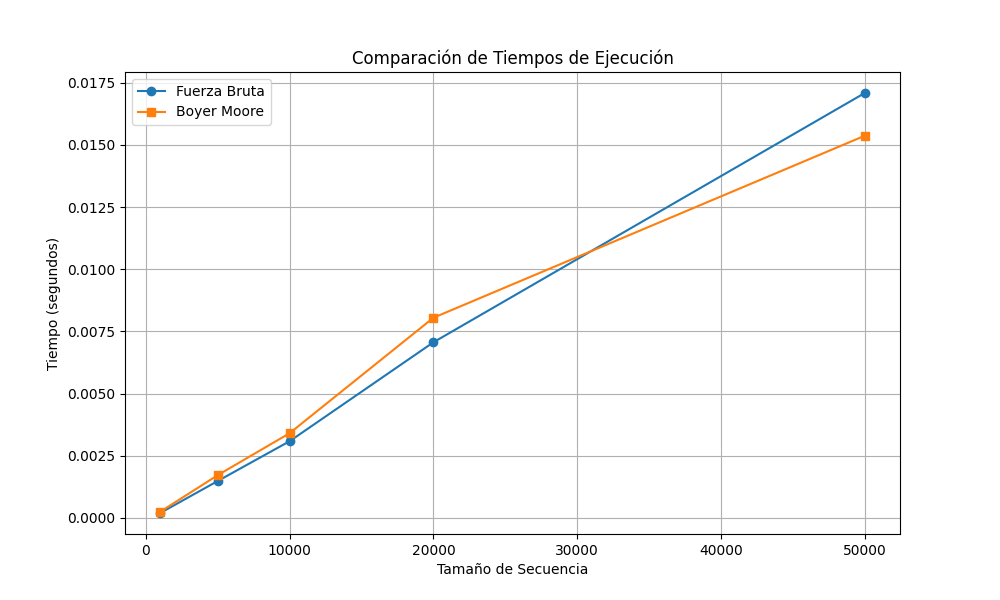
\includegraphics[width=0.7\linewidth]{grafico_comparacion.png}
    \caption{Comparación gráfica de tiempos de ejecución.}
    \label{fig:comparacion_tiempos}
\end{figure}

\subsection{Análisis}
Se observa en la Tabla \ref{tab:tiempos} y la Figura \ref{fig:comparacion_tiempos} que para secuencias pequeñas, la diferencia de tiempo entre Fuerza Bruta y Boyer-Moore es mínima, e incluso Fuerza Bruta puede ser ligeramente más rápido debido a la sobrecarga del preprocesamiento de Boyer-Moore. Sin embargo, a medida que aumenta el tamaño de la secuencia, el algoritmo Boyer-Moore tiende a ser más eficiente, como se evidencia en el caso de 50000 caracteres, donde supera a Fuerza Bruta. La eficiencia de Boyer-Moore depende de la naturaleza del patrón y del texto, permitiendo saltos más grandes y reduciendo el número total de comparaciones en casos favorables.

\section{Actividad 3: Búsqueda de Mutantes con Similitud}
Implementar un módulo que determine la posición de mutantes encontrados de un patrón en una secuencia de ADN, con un porcentaje de similitud mayor o igual al proporcionado.

\subsection{Comparación de Métodos (Ventajas y Desventajas)}
\begin{table}[h!]
    \centering
    \caption{Comparación de Métodos de Similitud}
    \label{tab:comparacion_metodos}
    \begin{tabular}{lp{4cm}p{4cm}p{4cm}}
        \toprule
        Algoritmo   & Ventajas                                      & Desventajas                                           & Recomendación de Uso \\
        \midrule
        Hamming     & \checkmark Rápido y simple. \newline \checkmark Eficaz para sustituciones. & \texttimes{} Solo funciona con cadenas de igual longitud. \newline \texttimes{} No detecta inserciones/deleciones. & Útil cuando las mutaciones son solo sustituciones (ej., SNPs). \\
        \addlinespace
        Levenshtein & \checkmark Detecta sustituciones, inserciones y deleciones. \newline \checkmark Más preciso para evolución molecular. & \texttimes{} Más lento computacionalmente. & Ideal para análisis detallado de mutaciones (ej., alineamiento local). \\
        \addlinespace
        N-gramas    & \checkmark Captura similitudes estructurales. \newline \checkmark Robusto a reordenamientos. & \texttimes{} Puede dar falsos positivos en secuencias repetitivas. & Útil cuando el orden exacto no es crítico (ej., dominios proteicos). \\
        \bottomrule
    \end{tabular}
\end{table}

\subsection{Umbral de Similitud Recomendado}
\begin{itemize}
    \item \textbf{Umbral conservador (pocos falsos positivos):} \(\geq 80\%\)
        \begin{itemize}
            \item \textit{Ejemplo:} Búsqueda de mutaciones patogénicas en genes clave.
        \end{itemize}
    \item \textbf{Umbral equilibrado (balance precisión/recall):} \(70-75\%\)
        \begin{itemize}
            \item \textit{Ejemplo:} Estudio de variantes evolutivas en secuencias homólogas.
        \end{itemize}
    \item \textbf{Umbral exploratorio (máxima sensibilidad):} \(\geq 60\%\)
        \begin{itemize}
            \item \textit{Ejemplo:} Screening inicial de mutaciones en regiones no codificantes.
        \end{itemize}
\end{itemize}

\textbf{Conclusión práctica:}
\begin{itemize}
    \item Levenshtein con umbral del 75\% es una opción robusta para la mayoría de los casos.
    \item N-gramas es útil para patrones complejos (ej., motivos regulatorios).
\end{itemize}

\subsection{Implementación Óptima}
\textbf{Ejemplo de uso con Levenshtein (recomendado):}
\begin{lstlisting}[style=pythonstyle, numbers=none, frame=none, backgroundcolor=\color{white}]
# Ejemplo de uso con Levenshtein (recomendado)
resultados = find_mutants(secuencia_ADN, patron, umbral=0.75, method='levenshtein')
\end{lstlisting}

\textbf{¿Por qué Levenshtein?}
\begin{itemize}
    \item Es el estándar en bioinformática para alineamientos locales (ej., BLAST).
    \item Considera todos los tipos de mutaciones relevantes en ADN (inserciones, deleciones, sustituciones).
\end{itemize}

\textbf{¿Cuándo usar otros métodos?}
\begin{itemize}
    \item \textbf{Hamming:} Si se buscan solo sustituciones y las secuencias tienen la misma longitud (ej., QC de secuenciación).
    \item \textbf{N-gramas:} Si el patrón tiene dominios repetidos o se busca similitud estructural más que secuencial exacta (ej., secuencias satélite).
\end{itemize}

\subsection{Código de búsqueda de mutantes}
\begin{lstlisting}[style=pythonstyle, caption={Búsqueda de mutantes con similitud}]
from typing import List, Tuple
from Levenshtein import distance as levenshtein_distance
from collections import defaultdict

def boyer_moore_preprocessing(pattern: str) -> Tuple[dict, list]:
    m = len(pattern)
    bad_char = defaultdict(lambda: -1)
    for i, char in enumerate(pattern):
        bad_char[char] = i
    good_suffix = [0] * (m + 1)
    suff = [0] * (m + 1)
    suff[m] = m
    for i in range(m - 1, -1, -1):
        if i > 0 and pattern[i] == pattern[m - 1]:
            suff[i] = suff[i + 1] + 1
        else:
            suff[i] = 0
    for i in range(m + 1):
        good_suffix[i] = m
    for i in range(m - 1, -1, -1):
        if suff[i] == i + 1:
            for j in range(m - i - 1):
                if good_suffix[j] == m:
                    good_suffix[j] = m - i - 1
    for i in range(m - 1):
        good_suffix[m - suff[i]] = m - i - 1
    return bad_char, good_suffix

def boyer_moore_search(text: str, pattern: str) -> List[int]:
    n, m = len(text), len(pattern)
    if m == 0 or n == 0 or m > n:
        return []
    bad_char, good_suffix = boyer_moore_preprocessing(pattern)
    positions = []
    s = 0
    while s <= n - m:
        j = m - 1
        while j >= 0 and pattern[j] == text[s + j]:
            j -= 1
        if j < 0:
            positions.append(s)
            s += good_suffix[0]
        else:
            bc_shift = max(1, j - bad_char[text[s + j]])
            gs_shift = good_suffix[j + 1]
            s += max(bc_shift, gs_shift)
    return positions

def hamming_similarity(s1: str, s2: str) -> float:
    if len(s1) != len(s2):
        return 0.0
    if len(s1) == 0:
        return 1.0
    mismatches = sum(c1 != c2 for c1, c2 in zip(s1, s2))
    return 1.0 - (mismatches / len(s1))

def levenshtein_similarity(s1: str, s2: str) -> float:
    max_len = max(len(s1), len(s2))
    if max_len == 0:
        return 1.0
    dist = levenshtein_distance(s1, s2)
    return 1.0 - (dist / max_len)

def ngram_similarity(s1: str, s2: str, n: int = 2) -> float:
    if n <= 0:
        raise ValueError("n debe ser positivo para n-gramas")
    def get_ngrams(s: str, n_gram: int) -> set:
        if len(s) < n_gram:
            return set()
        return set(s[i:i+n_gram] for i in range(len(s) - n_gram + 1))
    set1 = get_ngrams(s1, n)
    set2 = get_ngrams(s2, n)
    if not set1 and not set2:
        return 1.0
    if not set1 or not set2:
        return 0.0
    intersection = len(set1.intersection(set2))
    union = len(set1.union(set2))
    return intersection / union if union != 0 else 0.0

def find_mutants(C: str, P: str, S: float, method: str = 'levenshtein', n_gram_size: int = 2) -> List[List]:
    len_p = len(P)
    len_c = len(C)
    if len_p == 0 or len_c == 0 or len_p > len_c:
        return []
    exact_match_positions = boyer_moore_search(C, P)
    results = []
    processed_indices = set()
    for pos in exact_match_positions:
        results.append([pos, P, 1.0])
        processed_indices.add(pos)
    for i in range(len_c - len_p + 1):
        if i in processed_indices:
            continue
        kmer = C[i : i + len_p]
        sim = 0.0
        if method == 'hamming':
            sim = hamming_similarity(P, kmer)
        elif method == 'levenshtein':
            sim = levenshtein_similarity(P, kmer)
        elif method == 'ngram':
            sim = ngram_similarity(P, kmer, n=n_gram_size)
        else:
            raise ValueError("Método de similitud no válido. Usar 'hamming', 'levenshtein' o 'ngram'.")
        if sim >= S:
            results.append([i, kmer, round(sim, 4)])
            processed_indices.add(i)
    results.sort(key=lambda x: x[0])
    return results

def main():
    C_ejemplo = "CGCCCGAATCCAGAACGCATTCCCCTGGCCTCCATTCTGGAA CGGTACGGACGTCAATCAAAT".replace(" ", "")
    P_ejemplo = "ATTCTGGA"
    S_ejemplo = 0.625
    print(f"Secuencia C: {C_ejemplo}")
    print(f"Patrón P: {P_ejemplo}")
    print(f"Umbral S: {S_ejemplo}")
    print("-" * 30)
    print("Resultados usando Hamming:")
    mutantes_hamming = find_mutants(C_ejemplo, P_ejemplo, S_ejemplo, method='hamming')
    print(mutantes_hamming)
    print("-" * 30)
    print("Resultados usando Levenshtein:")
    mutantes_levenshtein = find_mutants(C_ejemplo, P_ejemplo, S_ejemplo, method='levenshtein')
    print(mutantes_levenshtein)
    print("-" * 30)
    print("Resultados usando N-gramas (n=2):")
    mutantes_ngram2 = find_mutants(C_ejemplo, P_ejemplo, S_ejemplo, method='ngram', n_gram_size=2)
    print(mutantes_ngram2)
    print("-" * 30)
    print("Resultados usando N-gramas (n=3):")
    mutantes_ngram3 = find_mutants(C_ejemplo, P_ejemplo, S_ejemplo, method='ngram', n_gram_size=3)
    print(mutantes_ngram3)
    print("-" * 30)

if __name__ == "__main__":
    main()
\end{lstlisting}
\begin{figure}[h!]
    \centering
    \includegraphics[width=0.5\linewidth]{qrlink.png}
    \caption{Código QR del repositorio en GitHub}
    \label{fig:qr_github}
\end{figure}

\noindent
Enlace al repositorio en GitHub: \url{https://github.com/lolalos/bioinformatica/tree/main/laboraa4}
\subsection{Resultados de ejemplo}
\begin{verbatim}
Secuencia C: CGCCCGAATCCAGAACGCATTCCCCTGGCCTCCATTCTGGAACGGTACGGACGTCAATCAAAT
Patrón P: ATTCTGGA
Umbral S: 0.625
------------------------------
Resultados usando Hamming:
[[6, 'AATCCAGA', 0.625], [7, 'ATCCAGAA', 0.625], [33, 'ATTCTGGA', 1.0]]
------------------------------
Resultados usando Levenshtein:
[[6, 'AATCCAGA', 0.625], [7, 'ATCCAGAA', 0.625], [32, 'CATTCTGG', 0.75], [33, 'ATTCTGGA', 1.0], [34, 'TTCTGGAA', 0.75]]
------------------------------
Resultados usando N-gramas (n=2):
[[32, 'CATTCTGG', 0.75], [33, 'ATTCTGGA', 1.0], [34, 'TTCTGGAA', 0.75]]
------------------------------
Resultados usando N-gramas (n=3):
[[32, 'CATTCTGG', 0.7143], [33, 'ATTCTGGA', 1.0], [34, 'TTCTGGAA', 0.7143]]
------------------------------
\end{verbatim}

\end{document}
